\documentclass[prb,preprint]{revtex4-1} 

\usepackage{amsmath}  
\usepackage{amsfonts} 
\usepackage{graphicx} 
\usepackage{color}
\usepackage{ulem}
\usepackage[T1]{fontenc}
\usepackage{mathptmx}
\usepackage{setspace}


\begin{document}
\begin{titlepage}
\thispagestyle{empty}
\begin{center}

\fontsize{20pt}{20pt}\text{   }
\vspace{30mm}

{\fontsize{18pt}{18pt}\selectfont \textbf{The Optical Production of Metastable Krypton Atoms \\ for the Development of the \\ Next Generation of Atom Trap Trace Analysis}}


\vfill
{\fontsize{14pt}{14pt}\selectfont \text{Danika Luntz-Martin}}

\vfill

\singlespacing{
Submitted to the Department of Physics \\
 of Smith College \\Ti:S
 in partial fulfillment \\
 of the requirements for the degree of \\
 Bachelor of Arts}



\vfill
{\fontsize{14pt}{14pt} \selectfont \text{William Williams,  Honors Project Advisor}}


\vfill
\fontsize{12pt}{12pt}{May 11, 2015}
\vfill

\end{center}
\end{titlepage}

\pagenumbering{arabic}

\section{Introduction} 

Radioactive dating is often the most effective method to determine the time at which an object originated. Radioactive carbon dating is a very popular method to date biological samples. However, radioactive dating is that limited by the half-life of the isotope used. At shorter times none of the atoms will have decayed, at longer time all of them will have. To date outside the range offered by carbon other atoms can be used. In this paper we address using krypton for radioactive dating.

The concept behind radiokrypton dating is the same as any other radioactive dating. The percentage the radioactive isotope is measured relative to the other isotopes of that atom. However, the mechanics of counting the relative numbers of each isotope is very different for different atoms. Carbon dating uses mass spectrometry to count the number of each isotope. Krypton dating requires a different method because \textcolor{blue}{remind me why this doesn't work for Krypton.} The method uses to date krypton is called Atom Trap Trace Analysis.

This senior thesis is the first year of a three year project designed to optically produce metastable krypton atoms for purposes of Atom Trap Trace Analysis.

\section{Theory}

Krypton is one of the noble gases; its outer electron shell is completely filled therefore the energy gap between the ground energy state and the first excited state is large. Therefore to laser cool from the ground state would require $123.5 nm$ light which is not currently experimentally possible. To be able to laser cool and trap krypton atoms they need to be in an excited state and that state needs to be metastable so that the atoms cannot decay while they are cooling and trapping them. Krypton has a metastable state that is $~80,000 cm^{-1}$ \textcolor{blue}{what is this?} $(~125 nm)$ above the ground state.  This metastable state, which is the lowest energy excited state, is doubly forbidden thus requiring three photons to transfer the atom from the ground state to the metastable state. \textcolor{blue}{We should talk about how it is doubly forbidden.} In order to optically create metastable krypton atoms, we choose to excite the atoms into a higher energy excited state using a two-photon transition at $215 nm$.  Once in this highly excited state, the atom can emit a photon (the third photon) and decay into the metastable state. 

To get the kryptons to the metastable state we used a $215 nm$ light to drive a two-photon transition from the ground $4p^6$ $^1S_0$ state, to the $5p_{[3/2]_2}$ state, see Figure~\ref{KrEnergyLevels}. Throughout our calculations we call the ground $4p^6$ $^1S_0$ state 'state 1' and the $5p_{[3/2]_2}$ state 'state 2.' There are other states at similar energies to the states in question, but they are not important for our experiment because the transitions are not resonant with our laser light, making it improbable for the atom to transfer to those states. From the $5p_{[3/2]_2}$ state the atom will either decay to an intermediate state and then ground state or it will decay to a metastable state, the $5s_{[3/2]_2}$ state. We called this metastable state 'state 3.' The last possibility is that the atom can ionize either from the the $5p_{[3/2]_2}$ state or the metastable $5s_{[3/2]_2}$ state. 

\begin{figure}[h!]
\centering
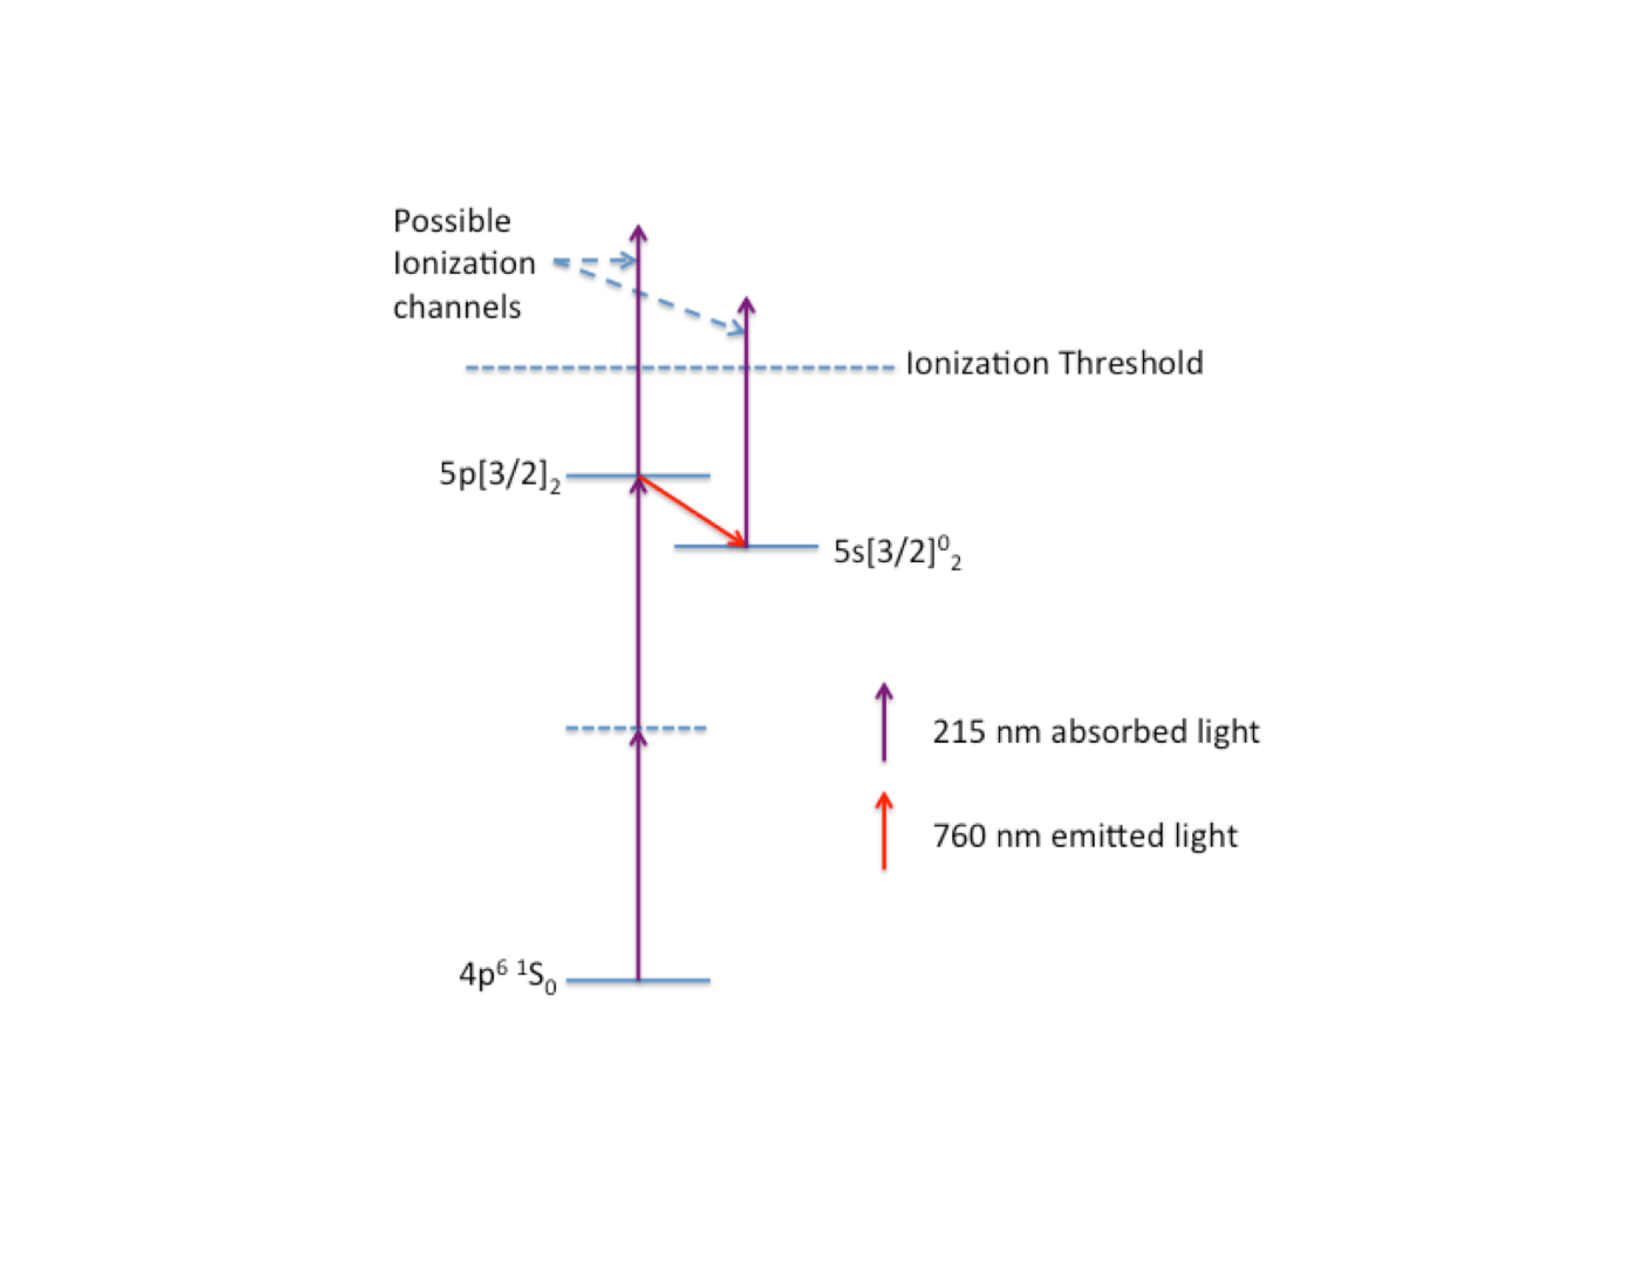
\includegraphics[width=6in]{KrEnergyLevels.pdf}
\caption{The energy levels of krypton. This figure only includes energy levels that are relevant to our experiment. Atoms are excited from the $4p^6$ $^1S_0$ state using two-photons to the $5p_{[3/2]_2}$ state then they decay either back to the $4p^6$ $^1S_0$ state or to the $5s_{[3/2]_2}$ state. Atoms can be ionized from both the $5s_{[3/2]_2}$ state and the $5p_{[3/2]_2}$ state.}
\label{KrEnergyLevels}
\end{figure}

Due to the isotope selectivity of laser cooling and trapping, Atom Trap Trace Analysis is able to count a specific isotope chosen by the laser frequency.  Only atoms in the metastable state can be trapped, so the efficiency of the apparatus is limited by the number of atoms transferred to the metastable state. To determine the efficiency of our set up, we calculated the percentage of krypton atoms that ended up in the metastable $5S_{[3/2]_2}$ state using the rate equations.

\begin{equation}
\label{RateEq1}
\frac{dN_1}{dt} = -\omega_{12}N_1 + \frac{1}{\tau_{21}}N_2
\end{equation}

Equation~\ref{RateEq1} gives the rate of change in the number of atoms ($N_1$) in the ground state. $\omega_{12}$ is the rate by which atoms in state 1 (the ground state) are excited to state 2, the $5P_{[3/2]_2}$ state, via the two-photon transition. The minus sign in front of $\omega_{12}$ indicates the atoms are leaving state 1. $\frac{1}{\tau_{21}}$ is the rate of decay from state 2 back to state 1. Similarly, there are differential equations for the three other states.

\begin{equation}
\label{RateEq2}
\frac{dN_2}{dt} = \omega_{12}N_1 -  \frac{1}{\tau_{21}}N_2 - \frac{1}{\tau_{23}}N_2 - R_2N_2
\end{equation}

\begin{equation}
\label{RateEq3}
\frac{dN_3}{dt} =  \frac{1}{\tau_{23}}N_2 - R_3N_3
\end{equation}

\begin{equation}
\label{RateEq4}
\frac{dN_4}{dt} = R_2N_2 + R_3N_3
\end{equation}

Where $\tau_{23}$ is the decay rate from state 2 to state 3, the metastable state. $\tau_{23}$ is the decay rate from state 2 to state 1, through an intermediary state. $R_2$ and $R_3$ are the ionization rates from states 2 and 3 respectively. $N_4$ is the number of atoms which have been ionized, just as $N_2$ and $N_3$ are the number of atoms in state 2 and state 3.

Solving these linearly dependent equations is possible, but the computational time is much shorter if they are put into matrix form.

\begin{equation}
\label{RateEqMatrix}
\begin{bmatrix}
	\frac{dN_1}{dt} \\
	\frac{dN_2}{dt} \\
	\frac{dN_3}{dt} \\
	\frac{dN_4}{dt} \\
\end{bmatrix}
=
\begin{pmatrix}
	-\omega_{12} & \frac{1}{\tau_{21}}  & 0 &  0   \\
	\omega_{12}  & -\frac{1}{\tau_{21}}- \frac{1}{\tau_{23}}-R_2 & 0 & 0 \\
	0  &  \frac{1}{\tau_{23}}  & - R_3 & 0 \\
	0  &  R_2  & R_3 & 0  \\
\end{pmatrix}
\begin{bmatrix}
	N_1 \\
	N_2 \\
	N_3 \\
	N_4 \\
\end{bmatrix}
\end{equation}

The general solution to the first order differential matrix equation is
\begin{equation}
\label{RateEqSol}
N(t) = A_1e^{\lambda_1 t} v_1 + A_2e^{\lambda_2 t} v_2 + A_3e^{\lambda_3 t} v_3 + A_4e^{\lambda_4 t} v_4 
\end{equation}

where $\lambda$ is an eigenvalue of the matrix and $v$ is an eigenvector of the matrix. $A$ is the amplitude determined by the initial condition. The initial condition is that all of the atoms are in the ground state, state 1. That is
\begin{equation}
\label{InitialCond}
N_1(0) = 1, \	\	\	\	
N_2(0) = 0, \	\	\	\	
N_3(0) = 0, \	\	\	\	
N_4(0) = 0 
\end{equation}

which allows us to obtain particular solutions to the rate equations. We did all calculations and analysis in Mathematica. Once we had the solutions to the rate equations we needed to define the variables $\omega_{12}$, $\tau_{21}$, $\tau_{23}$, $R_2$ and $R_3$ which make up the eigenvectors and eigenvalues of the matrix.

\subsection{Constant Intensity and Velocity Approximation} 

For our initial calculation we made a couple simplifying approximations. The first approximation we made was to model the intensity of the laser beam profile a step function.  Although the actual laser beam has a gaussian profile, this approximation allows for an exact solution to the above equations.  The height of the step function was constant and set equal to the maximum of the gaussian profile intensity. The width was set to twice the laser waist (also known as the laser radius) of the gaussian laser beam profile.  The second approximation was to assume all of the atoms in the collimated atomic beam were traveling with the root-mean-squared velocity of atomic beam's Maxwell velocity distribution.  The two approximations are standard in the community for evaluating the rate equations.  We later expanded our calculations to account for the gaussian beam profile and the velocity distribution; those calculations can be found in the subsequent sections. 

The decay rates for state 2 ($5P_{[3/2]_2}$) to state 1 (ground state) and state 3 (metastable state) are know quantities.~\cite{KrTransitions}
\begin{equation}
\label{DecayRates} 
\tau_{21} = 1.1x10^7 s, \	\	\	\	 \tau_{23} = 3.1x10^7s
\end{equation} 

The ionization rates are given by 
\begin{equation}
\label{IonizationRates}
R = \sigma_{pi} \frac{I}{\hbar\omega}
\end{equation}

where $I$ is the intensity of the laser calculated from power, $I = \frac{P}{\frac{1}{2}\pi w^2}$ and $w$ is the beam waist. We used a power value of $7.5 W$ based on a conservative estimate from the laser specifications. $\omega$ is the angular frequency of the light defined as $\omega = \frac{2\pi c}{\lambda}$. $\sigma_{pi}$ is the photo-ionization cross section, the probability that a photon will be absorbed by the atom. $\sigma_{pi2} = .5$ Mbarn for the $5p_{[3/2]_2}$ state and $\sigma_{pi2} = .25$ Mbarn for the $5s_{[3/2]_2}$ state.~\cite{Cannon} \textcolor{blue}{do I need to know more than that barn is a unit?}

The rate by which atoms are excited by two-photon transition from state 1 to state 2 is $\omega_{12}$ given by
\begin{equation}
\label{ExcitationRate}
\omega_{12} = \sigma_0\ g\ \frac{I^2}{(\hbar \omega)^2}
\end{equation}

$\sigma_0$ is the two-photon cross section, the probability that two photons will be absorbed, which is $4.4x10^{-35} cm.^{-4}$~\cite{NIST} $g$ is the on resonance line shape factor, defined as 

\begin{equation}
\label{LineShapeFactor}
g = 2 \sqrt{\frac{Log(2)}{2 \pi (\Delta \omega_L^2 + \Delta \omega_D^2)}}
\end{equation}

with $\Delta\omega_L$ as the line width of the laser. $\Delta \omega_D$ is Doppler line width for the two-photon transition, which is zero in our case because the krypton atoms are moving perpendicular to the laser.  The line shape factor becomes important whenever the line width of the transition is smaller than the line width of the laser.  When this happens, different frequencies of the light have different probabilities of exciting the atom.  The line shape factor, which is a convolution between the gaussian line shape of the laser and the Lorentzian line shape of the atomic transition, takes into account the varying transition probability across the frequency profile of the laser beam. 

The solution to these equations for $7.5 W$ of power inside the build up cavity is given in Figure~\ref{MetaGraph1} which shows the fraction of atoms in the metastable state as a function of the size of the laser's beam waist. The optimum number of atoms end up in the metastable state when the beam waist is close to 20 microns. When the beam waist is smaller than 20 microns more of the atoms are ionized since the intensity is large. When the beam waist is larger than 20 microns, the intensity is too small to drive the two-photon transition leaving most of the atoms in the ground state.

\begin{figure}[h!]
\centering
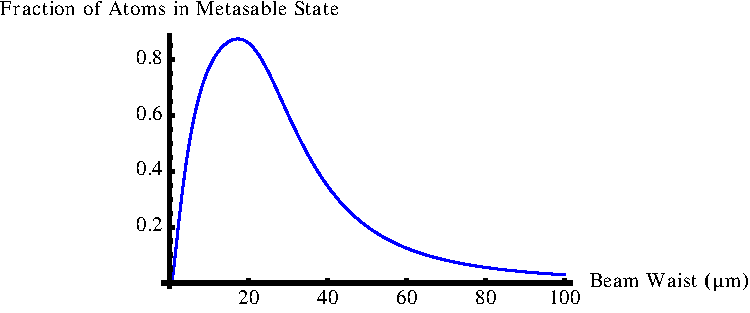
\includegraphics[width=6in]{MetaGraph1.pdf}
\caption{The fraction of atoms in the metastable state as a function of laser's beam waist. The fraction of atoms reaching the metastable state increases sharply as the beam waist increases until 20 microns. After 20 microns the number of atoms in the metastable state decreases because the intensity is too small.}
\label{MetaGraph1}
\end{figure}

Figure~\ref{TimeGraph} shows the fraction of atoms in each of the states as a function of time for a laser waist of $20 \mu m$, which is helpful to see how the atoms move between states. The maximum time of this graph is the atom-light interaction time given by the width of the step function (twice the laser waist) divided by the root-mean-square velocity of the Maxwell velocity distribution.  \textcolor{blue}{Is that true? I think this graph might be longer...} The green line is the ground state which starts at one because the initial condition is all of the atoms in the ground state and continuously decreases as time passes. The ground state, state 1 is the green line which decreases quickly as the atoms pass through the laser. State 2 is the orange line; it quickly increases as atoms are excited through two-photon transition. The number of atoms in state 2 decreases as atoms decay either back to the ground state or to the metastable state. The number of atoms in the metastable state increases as atoms decay to it from the state 2. Atoms only leave the metastable state if they ionize. For this laser waist, only a small fraction of atoms are ionized, see the red line.  It should be noted that the final number of atoms in the metastable state given in Figure~\ref{MetaGraph1} is the number of atoms in state 3 at the end of the atom-light interaction time (the last point on the plot in Figure~\ref{TimeGraph}) plus the fraction of atoms in state 2 that will naturally decay to state 3, about 74 percent.

\begin{figure}[h!]
\centering
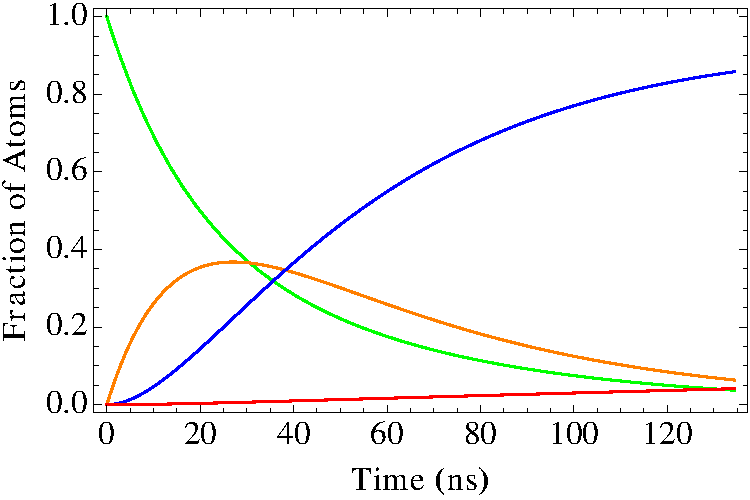
\includegraphics[width=6in]{TimeGraph.pdf}
\caption{The fraction of atoms in each state plotted against time. The green line is the ground state. The orange line is the excited $5p_{[3/2]_2}$ state. Blue is the metastable $5s_{[3/2]_2}$ and red is the fraction of atoms that have ionized.}
\label{TimeGraph}
\end{figure}

\subsection{Gaussian Beam Profile}

To make our model more accurate we factored in the intensity profile of the laser beam. From the laser manufacturer's, M Squared, specifications we know that the Ti:Sapphire laser's intensity profile is a two-dimensional gaussian. It was conceptually simple to incorporate the intensity profile into our previous calculation in place of the constant intensity. Computationally, it was not quite as easy.

We replaced our former intensity with by $I = I_0 e^{\frac{-2 x^2}{w^2}}$ where $I_0 = \frac{P}{\frac{1}{2}\pi w^2}$, the same intensity we used as a constant in our previous approximation. However, the addition of the gaussian term means that the equations no longer have analytical solutions. We solved the differential equations numerically.

The resulting graph is noticeably different from our first approximation, see Figure~\ref{AllGraph}. Adding the intensity profile does not change the shape of the peak, but it does make the peak lower and narrower. The location of the peak is now around 15 micrometers, rather than the 20 micrometers from the constant intensity approximation.  The fraction of atoms reaching the metastable state is still quite high having been decreased by just over five percent from roughly .9 to .85.

\begin{figure}[h!]
\centering
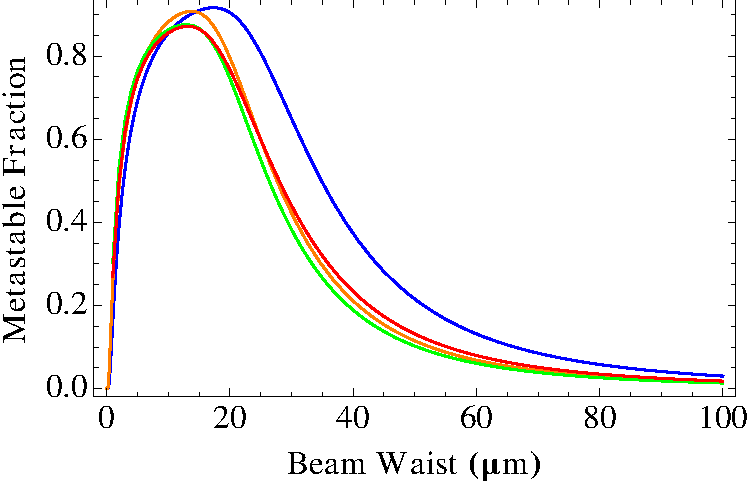
\includegraphics[width=6in]{AllGraph.pdf}
\caption{The blue line represents the calculation assuming all atoms have the same velocity (the root-mean-square velocity) and a constant intensity. The green line represents the calculation assuming the root-mean-square velocity and a gaussian intensity profile. Finally, the red line is the calculation using both the gaussian intensity profile and the Maxwell velocity distribution. The root-mean-square velocity is a good approximation; the green and red lines are very close. The constant intensity is not as good an approximation for the more accurate gaussian intensity profile, note the differences between blue line and the green line.}
\label{AllGraph}
\end{figure}


\subsection{Maxwell Velocity Distribution}

Adding the Maxwell velocity distribution presents new difficulties. To account for the range of velocities we first calculated the fraction of atoms in each of a series of velocity intervals. Then we calculated the fraction of atoms from each interval, that is from each different velocity range, that reach the metastable state. We then multiplied the fraction of atoms that reach the metastable state from a velocity interval by the fraction of atoms in that velocity interval. Then we added together the resulting fraction from each interval to obtain the total fraction of atoms that end up in the metastable state.  In other words, we evaluated the probability an atom gets transferred to the metastable state for all velocities and then weighted those probabilities according to the Maxwell velocity distribution.  See Figure~\ref{AllGraph} for a comparison of the fraction of atoms reaching the metastable state from each calculation.

Modeling the velocity of the atoms as the root-mean-square velocity is a very good approximation. The differences between using the root-mean-square velocity as a single average value and using the Maxwell velocity distribution were quite small. See the similarity between the green and red lines in Figure~\ref{AllGraph}.  This result gives us confidence that in future calculations we do not have to use the computation time to take into account the full Maxwell distribution.

\textcolor{blue}{You said you didn't understand this paragraph. We should probably talk about it, you added a sentence earlier which was saying the same thing I am trying to say here.}
The fraction of atoms reaching the metastable state is constant through time. The number of atoms that are in the metastable state at a specific time does change, look back to Figure~\ref{TimeGraph}. The number of atoms in the metastable state increases through time before plateauing. However the total fraction of atoms reaching the metastable is the fraction of atoms that are currently there plus the fraction of atoms in the excited, second state that will decay into the metastable state. The sum of these two numbers remains constant through time which is why our total calculation is stable through time.
  

\section{Titanium-Sapphire Laser}

A titanium-sapphire (Ti:S) laser uses titanium doped sapphire crystals as a lazing medium, hence the name. The crystal is placed inside a ring optical cavity, see Figure~\ref{InsideTiS}. The resonance length of the optical cavity is controlled by a birefringent filter and an etalon. The exact setup of the Ti:Sapphire laser from MSquared Lasers is proprietary, however the basic components are not. Ti:Sapphire crystals are made by doping $\text{Al}_2\text{O}_3$ with $\text{Ti}^{3+}$ ions which replace some of the $\text{Al}^{3+}$ ions.~\cite{Ti:S} Ti:S crystals are used because they have a broad range for absorption and emission of light. They can absorb light ranging from $~400 nm$ to $~600 nm$ and emit light from $~700 nm$ to $~1000 nm$.~\cite{Ti:S} Because the Ti:S emits so many wavelengths, to obtain monochromatic light the range of wavelengths is narrowed using a birefringent filter. Various wavelengths experience different transmission rate through the birefringent filter, rotating the filter selects for the desired wavelength. The birefringent filter is a rough selection, the band of wavelengths is still large (around 20 GHz). To further narrow the bandwidth the Ti:S uses an etalon.   By tuning the angle of the birefringent filter and etalon together, a single frequency mode with a width of about 5 MHz can dominate the resonance structure of the cavity.  Due to the exponential growth inside a lazing medium, this resonant laser mode dominates all other modes.  The optical diode in Figure~\ref{InsideTiS} is an optical element that stops the laser light from traveling the wrong direction in the cavity.  The crystal itself is pumped using a Coherent Verdi-V18, which is a diode-pumped laser emitting green $(532nm)$ light. The pump laser could be operated at various powers which adjusted the overall output of the Ti:Sapphire laser. We operated the pump laser at both 18 W and 12 W.

All the optical components in the SolsTi:S from M Squared are automated. The desired wavelength is selected on the laptop and the birefringent filter and etalon adjust automatically.

\begin{figure}[h!]
\centering
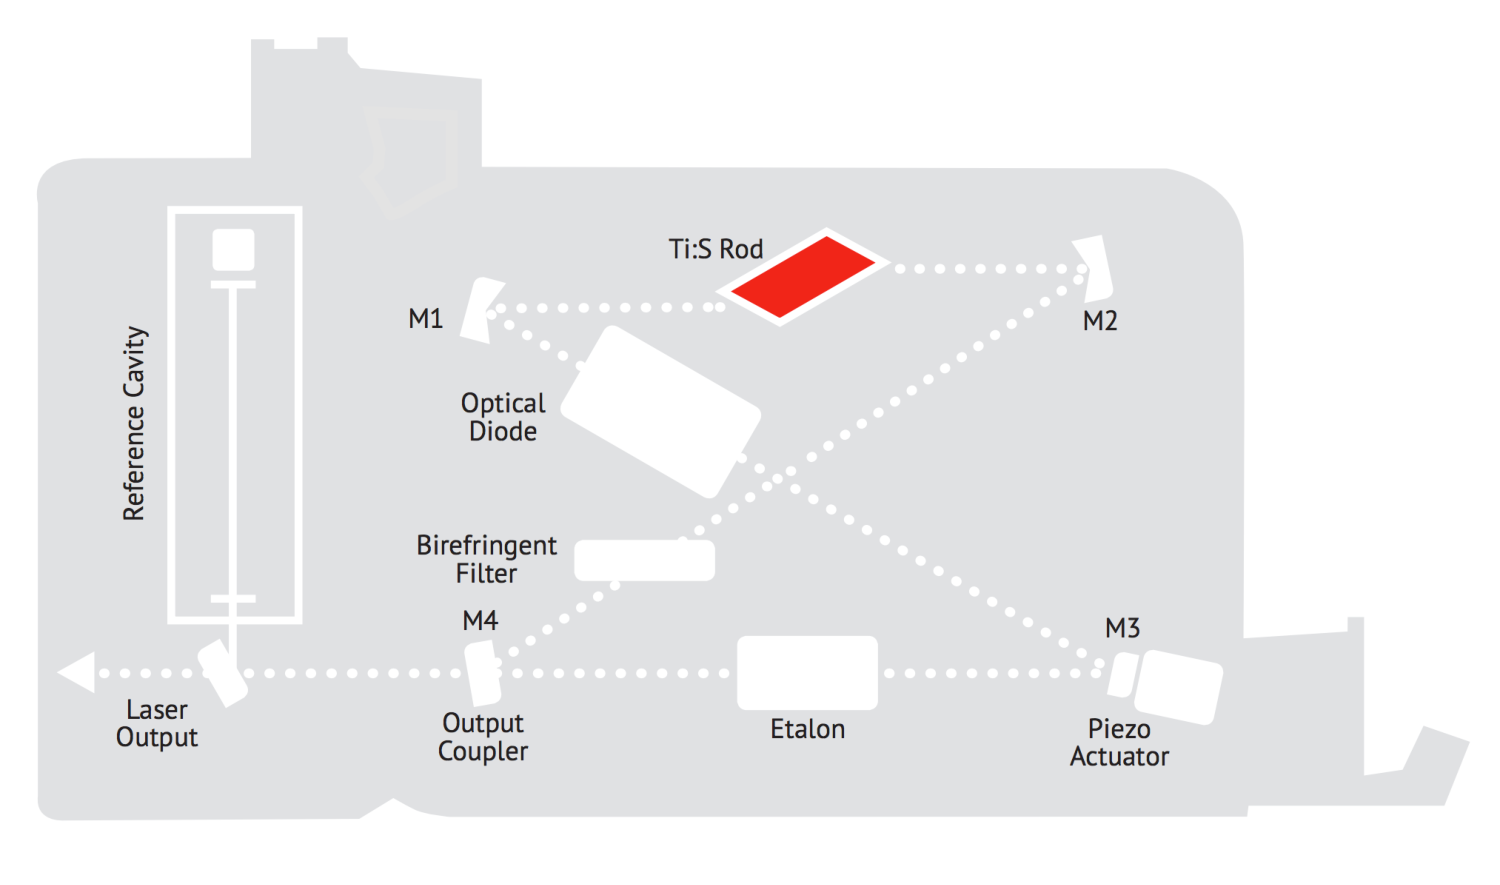
\includegraphics[width=6in]{InsideTiS.pdf}
\caption{}
\label{InsideTiS}
\end{figure}
The laser light exits the ring cavity through the output coupler.  This single mode light is then sent to the reference cavity.  The reference cavity is a confocal Fabry Perot cavity.  Since there are no optical elements in this cavity, the resonant length is simply whenever integer multiples of the laser wavelength fits nicely into the cavity.  In the confocal configuration, the resonant condition is $L=n \lambda/4$ where $n$ is an integer.  The purpose of this cavity is to further reduce the frequency width of the laser.  Once the etalon is locked to a particular lazing mode, which is discussed below, the laser can be stabilized to the reference cavity.  The resonance width of the reference cavity is less than 50kHz.  Once locked to the reference cavity, that signal can be fed back to the etalon.  This feedback signal can be used to correct the angle of the etalon further narrowing the frequency width of the laser to, at best, the resonance width of the reference cavity.  After stabilization to the reference cavity, the frequency width of the Ti:S laser is approximately 50 kHz.
Once both the etalon and reference cavity signals are stabilized, both the angle of the etalon and the length of the reference cavity can be changed simultaneously.  Moving the two optical elements together "pulls" the laser such that it is still resonant with both the ring optical cavity and the reference cavity.  This is how the Ti:S laser frequency is scanned in a controlled manner.  The scan range of this laser is approximately 25 GHz.
Other important laser parameters include amplitude noise, the spatial mode, the beam radius, and the beam divergence.  From the data sheet, the amplitude noise is less than $0.1\%$ RMS above the Verdi pump laser.  The output mode is the lowest energy spatial (Gaussian) mode, also known as the ${TEM}_{00}$ mode.  The beam radius is about $0.4 mm$ with a divergence of less than $1.5$ mrad.  Finally the output polarization is horizontal.

After the laser light leaves the main Ti:S laser, it then consecutively passes through two frequency doubling cavities. Refer to Figure~\ref{LaserSetup} for the experimental set-up of the laser.  Each doubling cavity is preceded by a beam splitter module and an alignment module.  The beam splitter module allows us to "pick-off" a portion of the laser light to use in another experiment or to monitor the laser.  The alignment module contains a mirror that allows us to spatially align the laser with the doubling cavity.  There is also a beam splitter module and beam alignment module between the pump laser and Ti:S laser.  This beam splitter module will be used in the beryllium experiment in a separate mixing cavity to produce 332nm light.  The alignment module is to optimize coupling into the Ti:S laser.

\begin{figure}[h!]
\centering
\includegraphics[width=6in]{LaserSetup.pdf}
\caption{The experimental set-up of the Ti:S laser comprised of a pump laser, Ti:S laser, reference cavity, doubler and quadrupler. Each component is separated by a beam splitter and a beam aligner, which consists of a set of mirror to adjust the beam along each axis.}
\label{LaserSetup}
\end{figure}

The doubling cavities behave very similarly to the ring cavity inside the Ti:S laser.  Instead of a titanium doped sapphire crystal, a strongly birefringent nonlinear crystal is used.  These crystals are capable of absorbing two photons and emitting a single photon with twice the energy.  As a result, the wavelength of light is cut in half while the frequency doubles.  A standard ?-Barium borate (BBO) crystal is used in the first frequency doubling cavity to convert $860$ nm light to $430$ nm light for the krypton project or to convert $940$ nm light to $470$ nm light for the beryllium project.  The ring cavity is not needed to double the frequency of the light.  Simply sending the light through the crystal once will convert some of the $860$ nm light into $430$ nm light.  The crystal is placed in the cavity allows many more opportunities for the light to be converted.  Also, since the crystal is nonlinear, the cavity provides a much higher intensity further increasing the efficiency of the doubling medium.  The second doubling crystal is very similar to the first, but uses a crystal designed to double $430$ nm light to $215$ nm light for the krypton project or to double $470$ nm light to $235$ nm light for the beryllium project.

\section{Operating Procedure}
The first step to operating the laser was to turn on the coolers which cooled the sapphire crystals and the pump laser and then to turn on the pump laser and allow it to warm up and stabilize. The pump laser takes around thirty minutes to warm up, before it is warm it will not generate any light from the Ti:Sapphire laser. It is preferable to allow the pump laser longer to fully stabilize because any drift in the pump laser will cause the Ti:Sapphire deviate from optimum and likely lose lock. After the pump laser is warm and stable, the shutter should be opened allowing light to pass into the Ti:Sapphire laser. The Ti:Sapphire crystals should be given ten to fifteen minutes to warm up before locking is attempted.

Once the Ti:Sapphire crystals are warm, the light from the pump laser into the Ti:Sapphire laser must be optimized. The the output from the pump laser passes first through a beam splitter, then through a set of mirrors which can be used to align the beam in all three axis directions. The power to the Ti:Sapphire laser can be measured by using the beam splitter after the Ti:Sapphire laser and reference cavity, again see Figure~\ref{LaserSetup} and a power meter. The alignment in the $z$ direction, the direction of propagation, should not be adjusted, but the horizontal and vertical directions, $x$ and $y$, should both be adjusted to maximize the output power of the Ti:Sapphire laser. After optimizing the pump laser into the Ti:Sapphire laser the output voltages can be examined on an oscilloscope and used for diagnostic purposes. 

The Ti:Sapphire laser from M Squared is controlled from a laptop using the provided software. The desired wavelength is selected on the laptop. After selecting the wavelength, the first step is lock the etalon. The etalon is locked at a point where its error signal crosses zero. The etalon error signal can be seen by selecting 'Etalon Error' from the dropdown menu for one of the monitors and scanning the resonator cavity continuously. The etalon error signal can be seen on the oscilloscope; if it is not symmetric around zero, the pump laser may need to be re-optimized into the Ti:Sapphire laser. A typical signal for the etalon error can be seen in Figure~\ref{EtalonError}. The etalon is then locked by clicking 'Apply Lock' on the computer. The locked signal should be a zero and show only noise. The signal to noise ratio for the etalon is 13. The locked voltage should be close to $100 V$, if the voltage on the laptop is not within $100 \pm 15 V$ the laser is not locked even if the software reports otherwise.

\begin{figure}[h!]
\centering
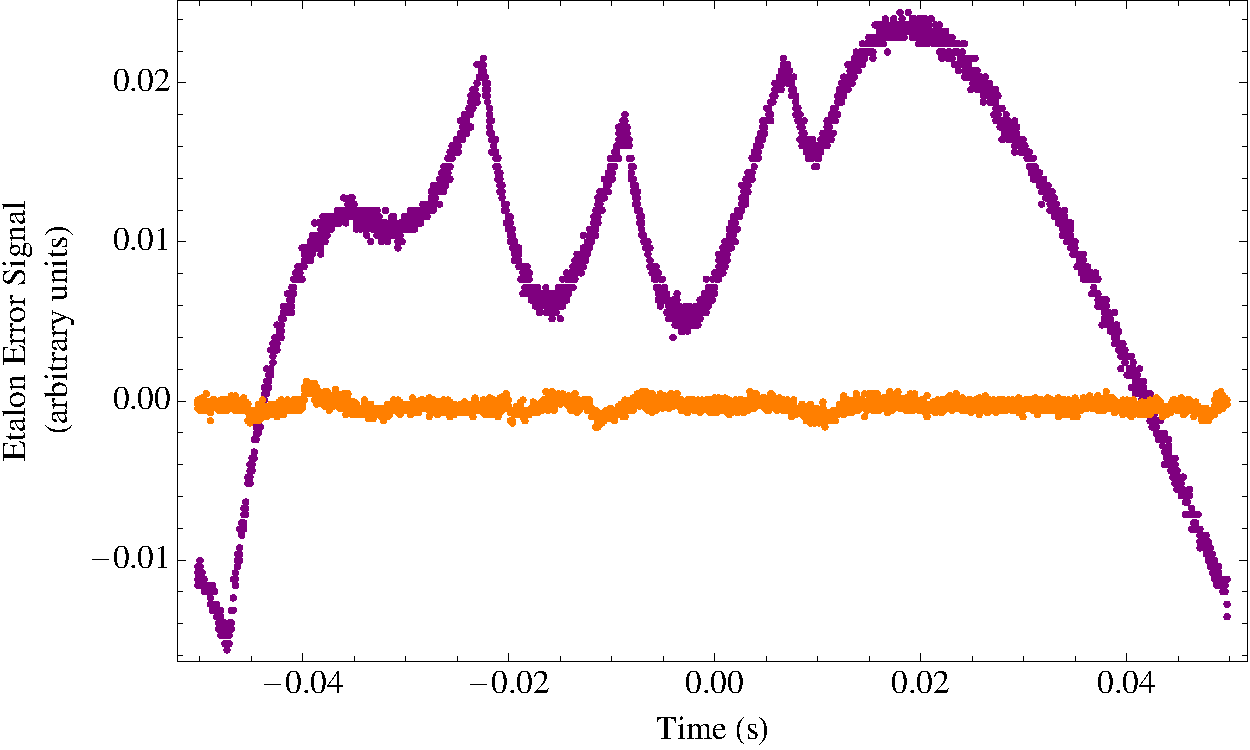
\includegraphics[width=6in]{EtalonError.pdf}
\caption{The etalon error signal as seen on the oscilloscope both before, maroon, and after, orange, the etalon has been locked. The signal to noise ratio is 13.}
\label{EtalonError}
\end{figure}

The second step of locking the Ti:Sapphire is the reference cavity. The reference cavity narrows  band of wavelengths produced by the laser. The reference error can be viewed on the oscilloscope by scanning the reference cavity continuously and selecting the reference error from the monitor menu. The reference error must cross zero to support a good lock, if the reference error does not cross zero it should be adjusted by clicking on the "PD Trim" button and a raising or lowering the "Ref Cavity PD Gain" in the pop-up window. Once locked the reference error should be zero on the oscilloscope and $100 \pm 15 V$ on the laptop. As can be seen in Figure~\ref{ResonatorError}, the signal error ratio for the reference cavity is large, 377.

\begin{figure}[h!]
\centering
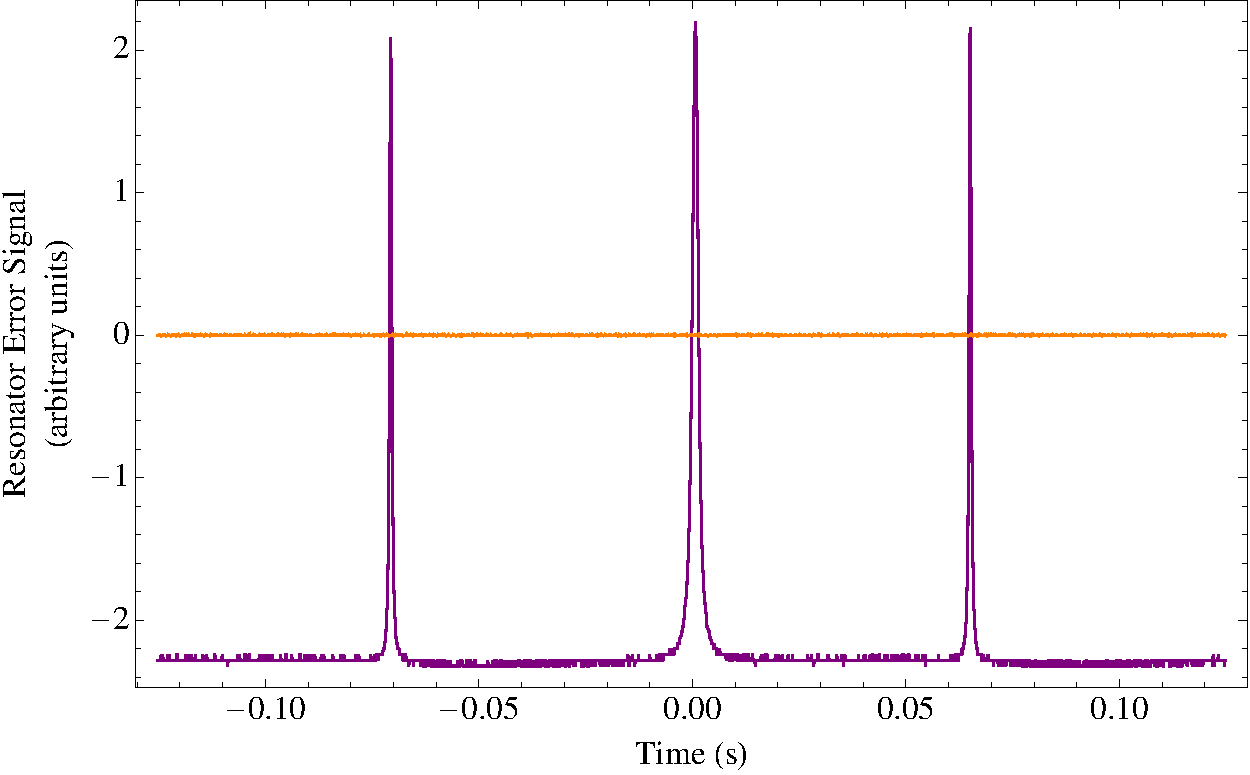
\includegraphics[width=6in]{ResonatorError.pdf}
\caption{The maroon line is the reference cavity error signal before it is locked and the orange line is after the resonator has been locked. The signal to noise ratio is 377.}
\label{ResonatorError}
\end{figure}

Next the laser light must be coupled from the Ti:Sapphire laser into the ECD-X, Ultra-compact Frequency Doubling Accessory. The light passes through a beam splitter and an arrangement of mirrors to adjust alignment before reaching the EDC-X, refer back to Figure~\ref{LaserSetup}. To optimize the light into the ECD-X, look at ``ECD PD 1'' on the oscilloscope and adjust the mirrors in the horizontal and vertical directions between the reference cavity and the ECD-X. The voltage of the ECD photo diodes (PD 1 and PD 2) should be optimized at the same mirror alignment, by maximizing voltage on the oscilloscope. After maximizing PD 1, confirm the alignment by checking that PD 2 is also maximized.

Experience has shown that ECD-X, the doubler, is the most difficult to lock. It is extremely sensitive instability in the etalon error and reference cavity error; if they are locked more than $8 V$ away from $100 V$ the ECD-X is unlikely to lock. The ECD error is the difference of the ECD photo diode signals. To see it on the oscilloscope select ``ECD error'' from the monitor menu and start a continuous scan of the ECD. An example of the ECD error, before and after it is locked, is in Figure~\ref{ECDError}. If the ECD does not cross zero, open the ECD adjustment window on the laptop by clicking ``ECD'' then adjust ``PD 1 gain'' and ``PD 2 gain'' until the ECD error signal crosses zero. The ECD usually requires a slight offset from zero to lock. If the ECD does not lock when the lock is applied, increase the ``Aux PD gain'' (also in the ECD window.) If the ECD is still not locking, the reference cavity and etalon should be unlocked, re-optimized and relocked. The ECD has a signal-to-noise ratio of 27.

\begin{figure}[h!]
\centering
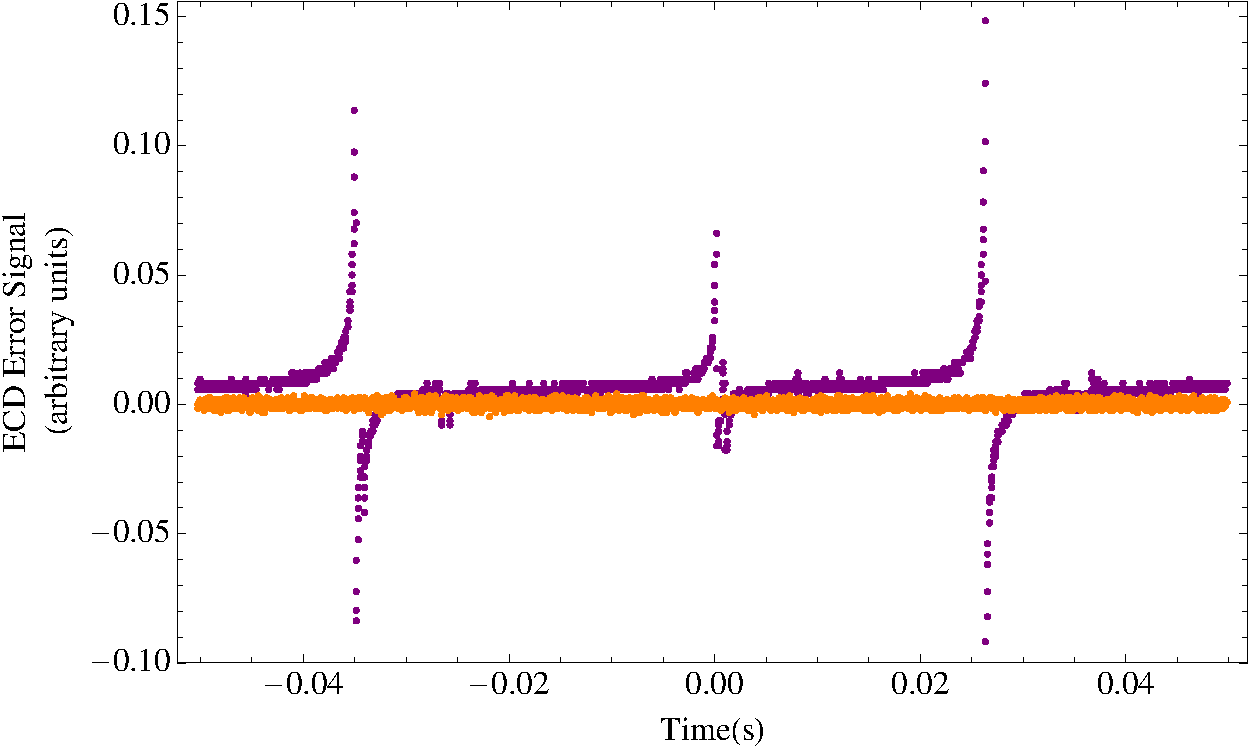
\includegraphics[width=6in]{ECDError.pdf}
\caption{The maroon line is the ECD error signal before it is locked, which is difference between PD 1 and PD 2. After it has been locked, the error signal is the orange line. The signal to noise ratio is 27.}
\label{ECDError}
\end{figure}

Once the doubler (ECD-X) has been locked the final step is locking the quadrupler (ECD-X-Q.) The process of locking the quadrupler is similar to the process of locking the doubler. The software required to control the quadrupler is a different package from the other sections of the laser, switch to the other control console on the laptop. Just like the doubler, the quadrupler is optimized by looking at PD 1 and PD 2 on the oscilloscope. They should be optimized by adjusting the beam alignment in the horizontal and vertical directions. The ECD-X-Q error can been seen on the oscilloscope and adjusted in the same manner as the ECD-X. It most cases the quadrupler will lock with more ease than the doubler. The locked and unlocked error signals can been seen in Figure~\ref{ECDQError}. The signal-to-noise ratio is comparable to that of the doubler at 20.

\begin{figure}[h!]
\centering
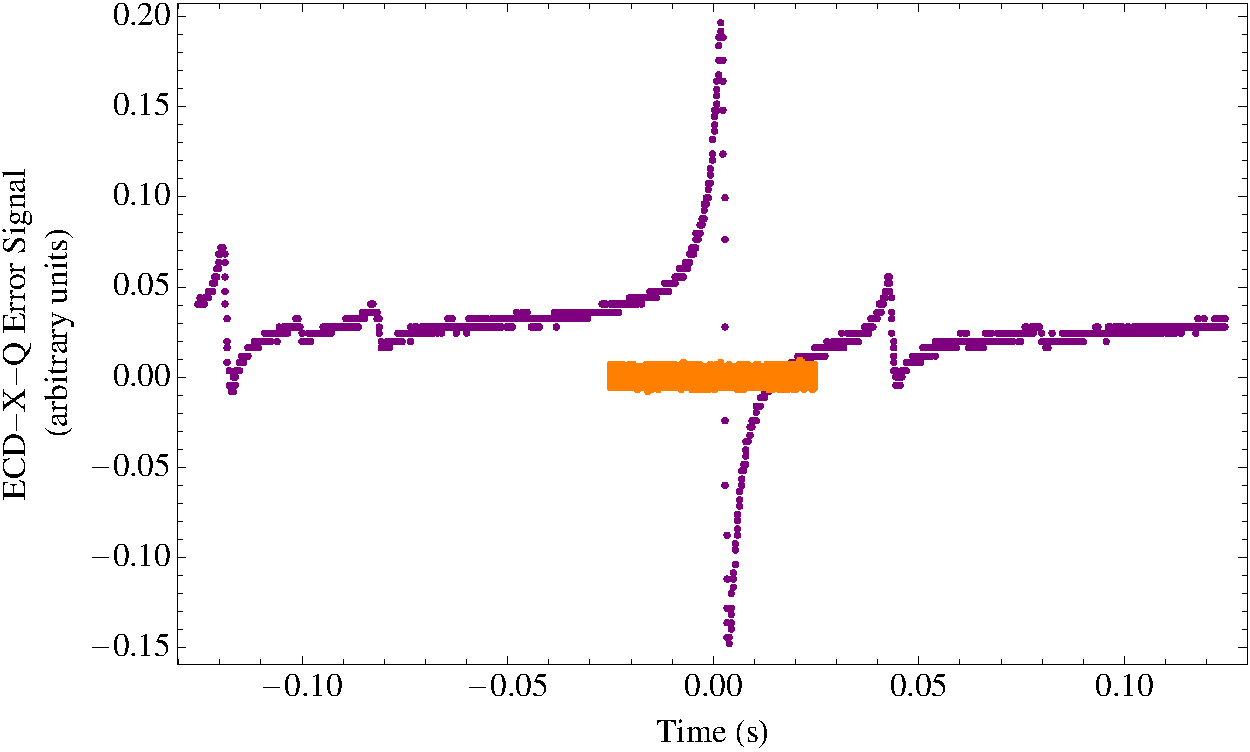
\includegraphics[width=6in]{ECDQError.pdf}
\caption{The maroon line is the ECD-X-Q error signal before it is locked, which is difference between PD 1 and PD 2. After it has been locked, the error signal is the orange line. The signal to noise ratio is 20.}
\label{ECDQError}
\end{figure}

The quadrupler lock is sensitive to vibration and likely to unlock. The reference cavity is more stable, but can also unlock particularly if the pump laser drifts. The lock voltages should be checked periodically while working with the laser to ensure that lock has not been lost. If the lock voltages on the laptop have a difference greater than $15 V$ from $100 V$ than lock has been lost even if the laptop does not read ``lock error.'' When the lock fails the laser should be unlocked and relocked, with re-optimization if necessary.

When turning off the laser all locks should be removed. Then the pump laser shutter should be closed, blocking all light into the Ti:Sapphire laser. Afterwards the pump laser can been cooled if the setup will not be used for an extended period.

\section{Laser Stabilization}

\section{Appendix}

\textcolor{magenta}{Put Mathematica notebooks here!}


\begin{thebibliography}{2}

\bibitem{NIST} A. Kramida, Yu. Ralchenko, J. Reader, J. and NIST ASD Team (2013). NIST Atomic Spectra Database (version 5.1), [Online]. Available: \url{<http://physics.nist.gov/asd>} [Wednesday, 15-Jan-201422:06:55 EST]. National Institute of Standards and Technology, Gaithersburg, MD.

\bibitem{KrTransitions} W. E. Ernst and E. Schulz-Gulde, ``Transition probabilities for Kr I lines from wall-stabilized arc measurements,'' Physica B+C 93, 136–144 (1978)

\bibitem{Cannon} B. D. Cannon, ``Model calculations of continuous-wave laser ionization of krypton,'' PNNL-12253 (1999)

\bibitem{Ti:S} M Squared Lasers Ltd, "SolsTiS - Narrow Lindwidth, Tunable CW Ti:Sapphire Laser User Manual" v10.3

\end{thebibliography}


\end{document}
